\subsection*{Esercizio 1}

Si richiede di costruire una matrice di connessione $B\in \mathbb{R}^{5 \times 5}$
relativa ad un web di 5 pagine rappresentato in Fig.~\ref{fig:web}.

\begin{figure}[htbp]
    \centering
    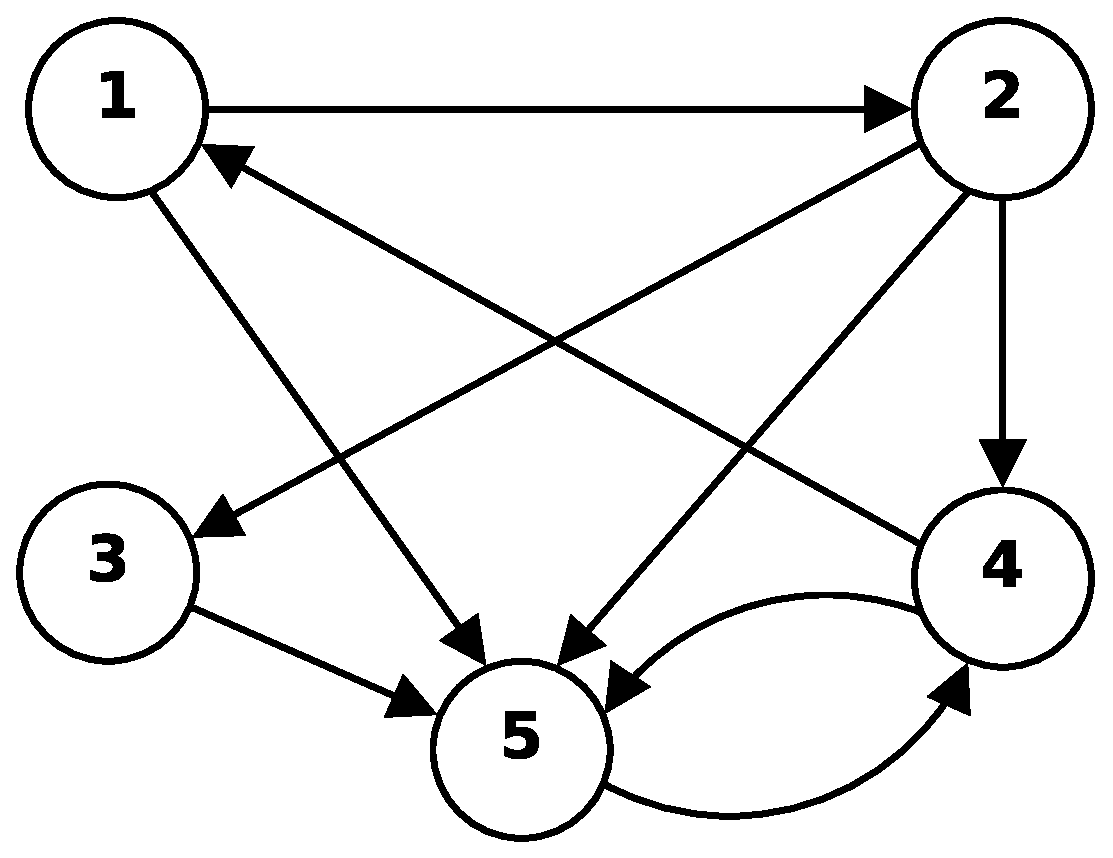
\includegraphics[width=0.4\textwidth]{./fig/web}
    \caption{Schema di un web di 5 pagine. Ogni cerchio rappresenta
    una pagina web, ogni freccia un link.}\label{fig:web}
\end{figure}

Utilizzando la libreria Eigen, si scriva una classe che permetta di calcolare
l'autovalore di modulo massimo (pari a 1) ed il corrispondente autovettore
(\emph{pagerank}). Si implementi anche l'operatore \cpp{operator <<} per
visualizzare a schermo i dati contenuti all'interno della classe.
